\documentclass[12pt]{article}
\usepackage[english]{babel}
\usepackage[english]{isodate}
\usepackage[table,svgnames]{xcolor}
\usepackage{url}
\usepackage[utf8x]{inputenc}
\usepackage[T1]{fontenc}
\usepackage{longtable}
\usepackage{amsmath}
\usepackage{graphicx}
\usepackage{parskip}
\usepackage{fancyhdr}
\usepackage{vmargin}
\usepackage{hyperref}
\usepackage{pgfgantt}
\usepackage{xparse}
\usepackage{float}
\usepackage{tabularx}
\usepackage{titling}
\usepackage[nogroupskip,toc,acronym]{glossaries}
\usepackage{fancyhdr}
\usepackage[authoryear]{natbib}
\usepackage{enumitem}
%\bibliographystyle{fontysIEEtranN}

\pagestyle{fancy}
\fancyhf{}
\lhead{
\includegraphics[width=0.2\linewidth]{TreewatchLogo.pdf}}
\rhead{Personal dossier Martijn Bonajo}
\rfoot{Page \thepage}

% alternate row colors for all tables
\definecolor{lightGrey}{rgb}{0.95,0.95,0.95}

\let\oldtable\table
\let\endoldtable\endtable
\renewenvironment{table}{\rowcolors{2}{lightGrey}{}\oldtable}{\endoldtable}

\let\oldtabular\tabular
\let\endoldtabular\endtabular
\renewenvironment{tabular}{\rowcolors{2}{lightGrey}{}\oldtabular}{\endoldtabular}

\let\oldtabularx\tabularx
\let\endoldtabularx\endtabularx
\renewenvironment{tabularx}{\rowcolors{2}{lightGrey}{}\oldtabularx}{\endoldtabularx}

\let\oldlongtable\longtable
\let\endoldlongtable\endlongtable
\renewenvironment{longtable}{\rowcolors{2}{lightGrey}{}\oldlongtable} {\endoldlongtable}

\graphicspath{{../img/}}

\renewcommand{\arraystretch}{1.5}

\DeclareDocumentCommand{\newdualentry}{ O{} O{} m m m m } {
  \newglossaryentry{gls-#3}{name={#5},text={#5\glsadd{#3}},
    description={#6},#1
  }
  \makeglossaries
  \newacronym[see={[Glossary:]{gls-#3}},#2]{#3}{#4}{#5\glsadd{gls-#3}}
}


\newlist{SMART}{description}{2}
\setlist[SMART]{leftmargin=12em,style=nextline}

\newlist{STAR}{description}{2}
\setlist[STAR]{leftmargin=8em,style=nextline}


%\loadglsentries{../glossary.tex}

\setmarginsrb{3 cm}{2.5 cm}{3 cm}{2.5 cm}{1 cm}{1.5 cm}{1 cm}{1.5 cm}

%\makeglossaries
\begin{document}

%%%%%%%%%%%%%%%%%%%%%%%%%%%%%%%%%%%%%%%%%%%%%%%%%%%%%%%%%%%%%%%%%%%%%%%%%%%%%%%%%%%%%%%%% Preface of the report

    \pagenumbering{roman} % Roman numerals for page counter


    % Title Page
    \begin{titlingpage}
        \begin{center}
            \begin{minipage}{\linewidth}
            \centering
            %University logo
            
\includegraphics[width=0.3\linewidth]{FontysLogo.pdf}
            \par
            \vspace{3cm}
            %Thesis title
            {\uppercase
                {\Large Personal dossier\\ Martijn Bonajo \\ 2015 Sofa GTL \\ TreeWatch Project
            \par
            \vspace{3cm}}}
            
\includegraphics[width=0.5\linewidth]{TreewatchLogo.pdf}
            \par
            \vspace{2cm}
            %Author's name
            {Martijn Bonajo\\
	         \par}
            \vspace{2cm}

            %Date
            \today
            \end{minipage}
        \end{center}
    \end{titlingpage}
    \clearpage

    \section*{Document information}
\addcontentsline{toc}{section}{Document information}
\renewenvironment{tabular}{\oldtabular}{\endoldtabular}
	\begin{tabular}{ll}
		\textbf{Document name:} & Personal dossier Martijn Bonajo\\
		\textbf{Document owner:} & Martijn Bonajo \\
		\textbf{Company/Organisation:} & Fleuren Baarlo \\
		\textbf{Contact person:} & Martijn Bonajo \\
		\textbf{Date:} & \today \\
		\textbf{Place:} & Fontys University of Applied Science Venlo \\
		\textbf{Author:} & \parbox[t]{5cm}{
		Martijn Bonajo\\ m.bonajo@student.fontys.nl\\ 2213297 \\}
	\end{tabular}
\renewenvironment{tabular}{\rowcolors{2}{lightGrey}{}\oldtabular}{\endoldtabular}

    %\printglossary[type=\acronymtype]
    %\printglossary
    \pagebreak

    %\listoffigures
    %\addcontentsline{toc}{section}{\listfigurename}
    %\listoftables
    %\addcontentsline{toc}{section}{\listtablename}
    %\pagebreak

    \tableofcontents
    \clearpage

%%%%%%%%%%%%%%%%%%%%%%%%%%%%%%%%%%%%%%%%%%%%%%%%%%%%%%%%%%%%%%%%%%%%%%%%%%%%%%%%%%%%%%%%% Main Part of the Report

    \pagenumbering{arabic}
    
    \section{Improving programming skills}
    
    This requirement was drafted when we thought we were going to develop using web technology and not via xamarin. So the requirement has changed from web based development to normal software development. \\
    I choose this one, because as a software engineer it is always good to keep improving your software skills, especially in new environments. For me it was new to develop for multi platform, so there is a lot to learn.
    
	\subsection{SMART learning goal}
	\begin{SMART}
	    \item[Specific] As a software engineer on this project I want to improve my programming skills. For this project this means I want to improve my web based programming skills.
	    \item[Measurable] Errors per kilo lines of code.
	    \item[Attainable] There are a lot of resources online on how to do the basic stuff.
	    \item[Relevant] This will improve my programming skills in web based applications, which will be useful when searching for a job as a software engineer.
	    \item[Time-limited]By January 2016, this project will be closed, therefore I will be able to manage the quality of a project until then.
	    \item[My complete goal] To improve my web based application development skills.
	\end{SMART}
	
	\subsection{STAR Analysis}
	\begin{STAR}
	    \item[Situation] We used Xamarin to create our multi platform application. For this project I was going to be one of the main developers. 
	    \item[Task] I wanted to improve my programming skills. Mainly on the multi platform aspect of this project. 
	    \item[Action] I worked on different features of our application during this project. From the shared code base in the Xamarin Forms, to the Android and iOS application. The first part I worked on was the field menu and the search bar inside the field menu. This is done by using the MVVM pattern to split GUI, program logic and data. The view can be found at CODEREF-MAPMENUVIEW and the the viewmodel can be found at CODEREF-MAPMENUVIEWMODEL. After this I started working on adding annotations and info windows on top of the map. This functionality is removed in a later stage of the application, because it was no longer needed. I continued working on the map, this time I wrote code that would zoom in when a specific field was selected, so that it was completely visible in the view and took up most of the view. The code for this can be found at CODEREF-MAPRENDERER. After this i started working on the Notes page inside our application, for this I added a plugin from Xamarin Forms Lab, which can be found at \url{https://github.com/XLabs/Xamarin-Forms-Labs/wiki/Camera}. This functionality has not yet been added to the master branch, because it has not been tested. After a little detour to the Notes page I went back to the map to add functionality to center on user position when a button is clicked and when the map is loaded for the first time. The code for this can be found in CODEREF-MAPRENDERER. For the biggest part I worked the Geofencing part of the application. First I made my own design to get geofencing to work cross platform, but after some testing I couldn't get it to work. After some research I found a plugin which had multi platform support for geofencing. This plugin is however outdated, but the design was still useful for me. The code for geofencing can be found at CODEREF-GEOFENCING.
	    \item[Result] I learned a lot by developing for multiple platforms. The measurement as can be seen in figure ~\ref{lgprogramming} there is no real improvement at the beginning of the application, because there still was a lot of new concepts every time. But after about half way through the project there is a slight improvement in the errors per 100 lines of code.
	    \item[Reflection] I think I did a good job on the programming part. I learned a lot about coding for different platforms, looking at the different api's and try to get most of it to work in an uniform way.
	\end{STAR}
	
	\begin{figure}[ht]
		
		\centering
		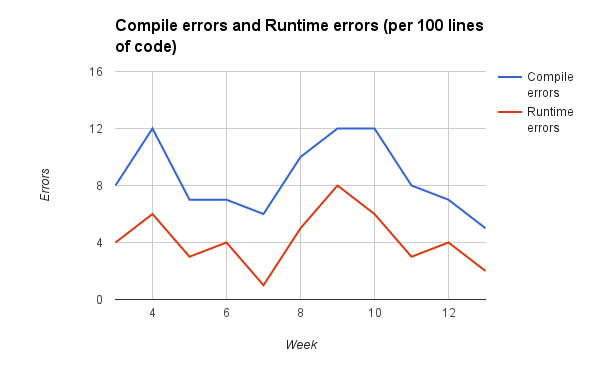
\includegraphics[width=\textwidth, keepaspectratio=true]{personaldossiers/LearningGoalProgrammingMartijn.png}
		\caption{Learning goal programming progress}\label{lgprogramming}
	\end{figure}
	
	\clearpage
	\section{Improve software design skills}
	\subsection{SMART learning goal}
	\begin{SMART}
	    \item[Specific] I want to improve my software design skills in this project.
	    \item[Measurable] Feedback on the design. Do this once halfway the project and once at the end of the project and check the difference between the amount of feedback.
	    \item[Attainable] There are a lot of resources online on how to make good software design.
	    \item[Relevant] Good software needs to start with a good software design.
	    \item[Time-limited] By January 2016, this project will be closed, therefore I will be able to manage the quality of a project until then.
	    \item[My complete goal] Improve my software design skills.
	\end{SMART}
	
	\subsection{STAR Analysis}
	\begin{STAR}
	    \item[Situation] We used Xamarin to create a multi platform application, this meant that the code should be able to run on both Android and iOS. Making designs for the code could help in these scenario to understand better what should be done for each platform.
	    \item[Task] I want to improve my design skills during this project. Both for code and database.
	    \item[Action] For this project we used the MVVM pattern, which is a software design pattern. An example of code I worked can be found at CODEREF-MAPMENUVIEW. For the database I helped working on the design for the database. The design for the database can be found at ER-DIAGRAM. Finally I made a design for the geofencing part of the application. Which can be found at GEOFENCE-DIAGRAM.
	    \item[Result] The GUI part of the application has where possible been done with the MVVM pattern. The database design is in use by the application. The geofencing design is implemented in the application and in use.
	    \item[Reflection] Most of the code has been written without first creating some kind of design, so there is still a lot of room for improving my design skills. I think the designs that have been made are of good quality.
	\end{STAR}
	
	\section{Improve logging skills}
	
	\subsection{SMART Learning Goal 3}
	\begin{SMART}
	    \item[Specific] I want to improve my logging skills.
	    \item[Measurable] How many times I am late or forget to log my activities. In the scrum tool it is possible to see if i didn't log my activities or if I was to late. So there is a way to check how many times this happens per week.
	    \item[Attainable] We use scrum board online where you can keep track of your tasks.
	    \item[Relevant] This is relevant for all projects, because you need to know what work is done and when this work was done.
	    \item[Time-limited] By January 2016, this project will be closed, therefore I will be able to manage the quality of a project until then.
	    \item[My complete goal] Improve my logging skills.
	\end{SMART}
	
	\subsection{STAR Analysis 3}
	\begin{STAR}
	    \item[Situation]
	    \item[Task]
	    \item[Action]
	    \item[Result]
	    \item[Reflection]
	\end{STAR}
	
	\begin{figure}[ht]
		\centering
		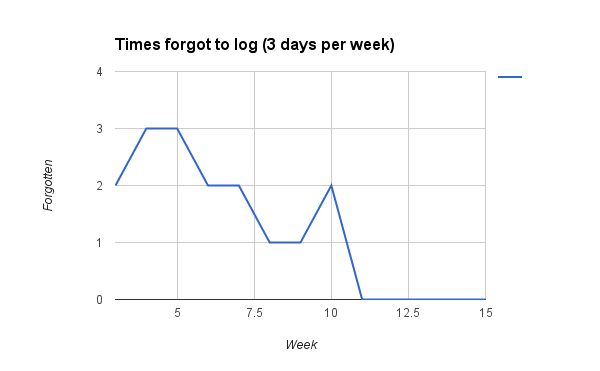
\includegraphics[width=\textwidth, keepaspectratio=true]{personaldossiers/LearningGoalLoggingMartijn.png}
		\caption{Learning goal programming progress}\label{lglogging}
	\end{figure}
	
	%\clearpage
	
	%\bibliography{biblist}
	
	\end{document}
